\section{Iterative design process}

To understand how to meet the needs of Herbie's users,
  after reviewing user-submitted bug reports,
  testing changes to the existing Herbie user interface,
  and mocking up a new interface,
  we conducted an iterative user design study.
As we observed users working with the prototype,
  we identified new needs and added features
  to meet those needs.
% Each phase generated observations and hypotheses
%   about Herbie users' needs and workflows,
%   which ultimately lead to the design of Odyssey.

% \subsection*{Phase 1: Analyzing Herbie's Usage and Issues}

% We began by reviewing 97 bug reports 
%   submitted by Herbie users,%
%   \footnote{Publicly available at \url{https://github.com/herbie-fp/herbie/issues}.}
%   and the developers' responses.
% After filtering out bug reports
%   about crashes or installation difficulties,
%   we were left with 24 bug reports
%   where Herbie was unable to meet
%   the user's floating-point error-improvement needs.
% We then grouped these issues
%   into three clusters of usability issues
%   with some reports belonging to multiple clusters. 

% First, in nine bug reports
%   (e.g., issues \#247, \#333), 
%   users are surprised that Herbie's output
%   gives a less accurate answer on specific inputs,
%   even though Herbie reports an overall improvement.
% In their response to these issues, 
%   Herbie developers explain that Herbie 
%   improves average accuracy over a range of input values, 
%   which might involve decreasing the accuracy for
%   specific inputs.
% For this cluster, we hypothesized that users would have benefitted
%   from a clearly indicated ``input range'' parameter for Herbie. 

% Second, in eight bug reports
%   (e.g., issues \#437 and \#391)
%   users asked why Herbie made certain complicated,
%   often meaningless, modifications to their program.
% In many of these bug reports,
%   the Herbie developers respond
%   that Herbie makes many decisions ``at random,''
%   and that users could use Herbie's derivations feature
%   to confirm whether a certain change
%   improved accuracy or not.
% We hypothesized
%   that making Herbie's derivation feature more prominent
%   would help users look at intermediate steps
%   to understand Herbie's decisions and pull out ``main ideas'' 
%   they can understand and maintain.
  
% Third, in 13 bug reports
%   (e.g., issues \#247 and \#261)
%   users asked why Herbie failed to find a specific modification users had in mind.
% In most of these bug reports,
%   the Herbie developers respond
%   that Herbie is missing certain ``rewrite rules''
%   or needs an internal parameter called ``num-enodes'' increased,
%   which would allow it to find more rewritings.
% We hypothesized that users needed more intuitive ways to guide Herbie's search
%   in order to find sensible rewritings for their applications.

% Reviewing the bug reports led us to observe the following: 
%  \begin{itemize}[label=$\circ$]
%    \item Users want to optimize solutions for limited input ranges relevant to their own needs.
%    \item Users want to understand why automated tools choose the rewritings they do, especially when the rewritings conflict with their own goals for an expression.
%    \item Users want to communicate their own rewriting ideas to automated tools to help shape the search process.
%  \end{itemize}

% The Herbie developers confirmed that they were aware
%   of the clusters of bugs we identified and had similar hypotheses. 
% For example, the Herbie team had recently 
%   added an option for user-specified input ranges, 
%   though it was hidden behind an ``advanced options'' panel. 
% Given our hypothesis about the importance of input ranges,
%   we designed and contributed an interface
%   that allowed users to more easily provide input ranges.
% This was merged into Herbie and released, 
%   along with the Herbie developers' other improvements, 
%   as Herbie 1.6.

% \subsection*{Phase 2: Testing the User Interface Changes}

% After the release, we continued monitoring the Herbie issue tracker.
% To our surprise, the changes made in Herbie 1.6
%   did not seem to significantly change issues users faced.

% While users \textit{were} explicitly specifying input ranges,
%   the user-specified input ranges were usually extremely wide,
%   often as wide as Herbie's default input ranges.
% Most users clearly did not have a small, domain-specific input range in mind. 
% Instead, users had both a large
%   range of possible inputs they wanted to visualize 
%   and several critical ranges
%   where they additionally checked for accuracy.


% Meanwhile, the Herbie developers experimented
%   with additional rewrites rules and larger ``num-enodes'' values
%   (published in~\cite{ruler} and~\cite{egg})
%   to try to find the expressions users were suggesting.
% However, these changes
%   did not solve Herbie's problems with finding user-suggested rewrites:
%   user rewrites might not be more accurate,
%   and Herbie found it difficult to optimize
%   for ``simplicity'' or ``maintainability'' automatically.
% We hypothesized that
%   if users could enter variations of Herbie's outputs themselves
%   and have Herbie \textit{validate} those programs,
%   they might feel more comfortable using and modifying Herbie's output,
%   even if Herbie's initial results did not meet their needs.
% Significantly, this would require extending the user interface
%   to allow the user to input and compare multiple programs.

% In other words, we made the following key observations: 
% \begin{itemize}[label=$\circ$]
%   \item Users want to check the performance 
%     of solutions both overall and on a variety of 
%     \textit{critical ranges}.
%   \item Despite improvements in automated methods, 
%     automated search will still sometimes fail 
%     to find the results users want. 
%     Users should have ways to submit and validate 
%     their own attempts at a solution.
%   \item In order to see the effects of their changes, 
%     users need ways to track and compare multiple rewritings.
% \end{itemize}

% To more rapidly iterate on user interface designs,
%   we began designing Odyssey as a new interface separate 
%   from Herbie's default user interface.\footnote{Coincidentally, around this time,
%   the developers informed us of a new mode for Herbie~\cite{pherbie}
%   designed to suggest multiple possible rewritings to the user.
% Since Odyssey already needed to support
%   tracking and comparing multiple rewrites,
%   we designed Odyssey to use the new mode as its default.}


% \subsection*{Phase 3: Presenting a Mock-up to FP Experts}

% To get early feedback on Odyssey,
%   we demonstrated a mock-up at the FPBench Community Meeting~\cite{fpbench-cm}.
% FPBench is a community of floating-point researchers,
%   including both the Herbie developers and the developers
%   of other floating-point analysis tools. 
%   The Community Meeting is a monthly Zoom call
%   where community members share progress,
%   discuss applications, and brainstorm new research directions.
% In our presentation,
%   we demonstrated how Odyssey
%   allowed users to see, track, and compare suggestions from Herbie;
%   enter their own programs;
%   and check the accuracy of a solution for different input ranges.
% FPBench community members were supportive.
%   Several community members wanted to use Odyssey
%   with their own floating-point systems as backends. 

% Numerical methods experts, 
%   who would be potential users of Odyssey, 
%   critiqued our assumption that users
%   would be able to find their critical ranges based on a visualization.
% The experts pointed out that 
%   the critical ranges they were typically interested in 
%   were too small to see in the chart.
% Based on this early feedback,
%   we added support for coordinated zooming,  
%   where users can type in a critical ranges, 
%   and Odyssey would simultaneously modify
%   its sampled inputs, visualizations, and accurate evaluations
%   to draw from the new range.

% Engaging with the FPBench Community led to the following observations:
% \begin{itemize}[label=$\circ$]
%   \item Users need to use a variety of visualization and generation
%     tools that do not currently interoperate.
% \end{itemize}

% Based on the positive feedback from the FPBench community,
%   we moved on to conduct a user design study
%   with FPBench community members.

\subsection*{User Design Study with Prototype}

Our user design study consisted of nine interviews
  with participants ranging from floating-point novices to experts.
Most participants were graduate students
  working on floating-point-related research
  with at least two years of experience.
We spaced these interviews out
  and iteratively added features to Odyssey,
  responding to user concerns after each interview.
% This phase reinforced some of our previous observations
%   and led to new observations.
We made the following observations.

% \newcommand{\phaseTwo}{Phase 2-Testing UI Changes~}
% First, we found that users would frequently
%   zoom the chart to specific critical ranges
%   and would interactively shift
%   between the full input ranges and critical subranges.
% (For an example, see~\Cref{fig:tuning}C.)
% One particularly interesting use of this feature
%   was for adjusting branch conditions.
%   For example, if Herbie suggested
%   an ``if $x < 0.1$'' condition,
%   users zoomed to the region between 0.01 and 1
%   and checked whether 0.1 was the best threshold.
% Users then modified the constant
%   and compared the accuracy of the modified program
%   thanks to Odyssey's support for comparing multiple 
%   user-submitted programs.

% We also made the following new observations.
First, we found that more experienced users
  iteratively submitted many hand-written programs to Odyssey.
In some cases, users modified a Herbie result,
  used Odyssey's reported error to confirm
  that the change didn't harm accuracy,
  and then used the modified program
  as a base for further modifications.
In other cases, users modified a Herbie result
  and re-ran Herbie on the modified expression,
  helping Herbie around a road-block of some kind
  and achieving a lower error as a result.
We also saw users combining pieces of different programs
  into a single final program.
Users described implicit trade-offs,
  for example noting that Herbie's result was very complex,
  and that deleting certain terms from Herbie's result
  was less accurate but easier to read.


\begin{figure*}
  \centering
  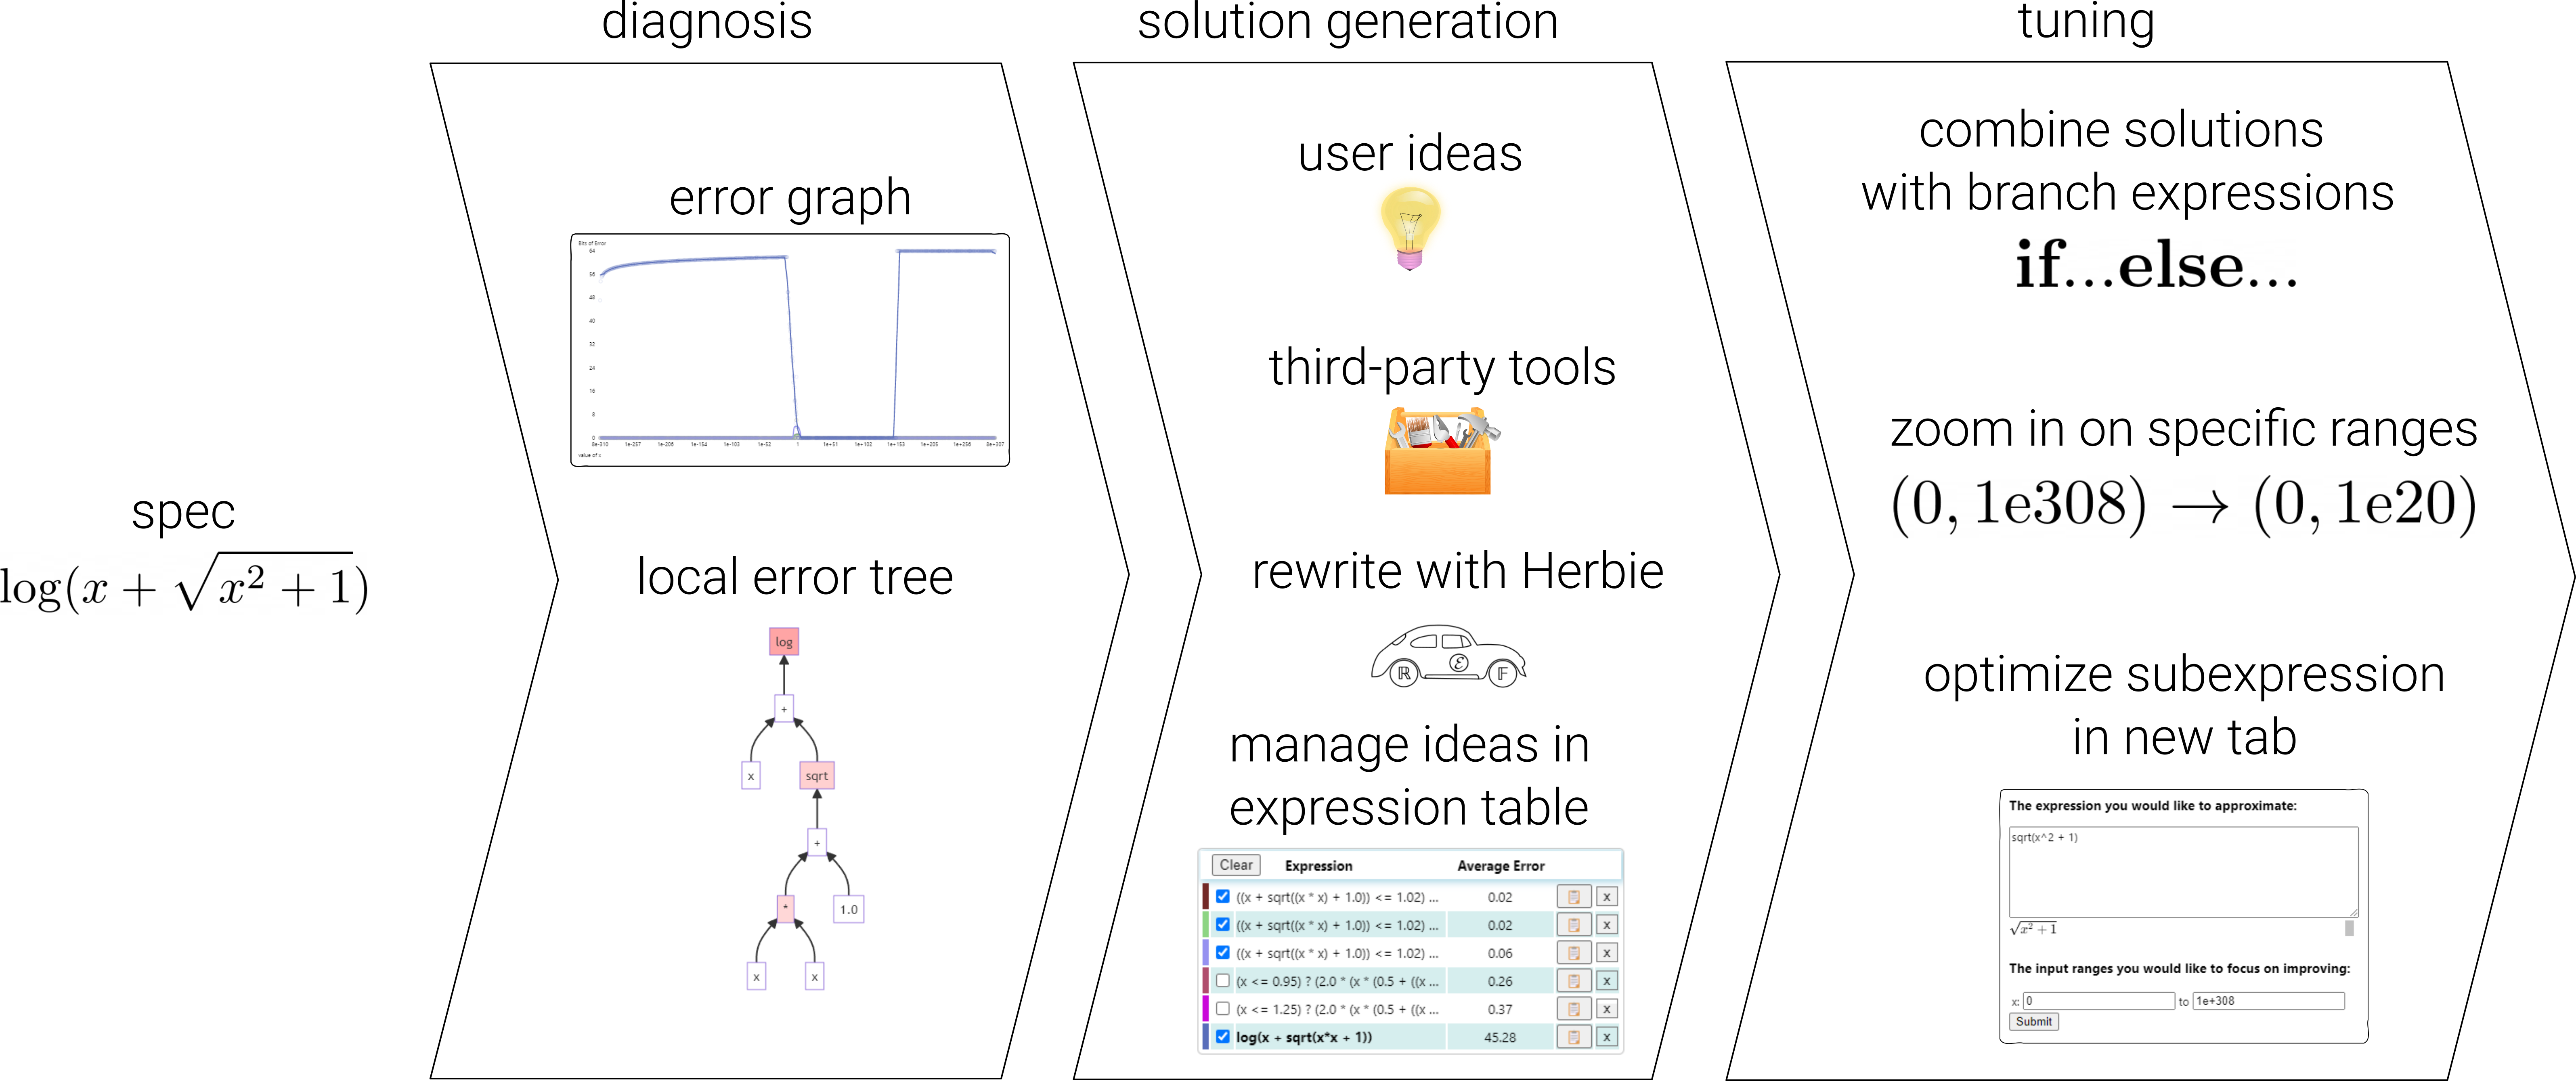
\includegraphics[width=\linewidth]{figures/workflow-diagram.png}
  \caption{The general workflow supported by Odyssey.
  Odyssey starts with a real-number specification,
    analyzes sources of error,
    creates different solutions based on the analysis,
    and tunes solutions based on user's needs.
  }%
  \label{fig:workflow}
\end{figure*}

Second, we noticed that many participants,
  including both novices and experts, 
  struggled to explain \textit{why} there was error in an expression,
  even when they could see the error in Odyssey's error plot.
For example, in the program $\log(x + \sqrt{x^2 + 1})$,
  most users could guess
  that the error for large $x$ values was caused by overflow, but
  far fewer participants could identify that error for small $x$
  was caused by the $\log()$ operation.

  In a follow-up conversation with the Herbie developers,
  we learned that Herbie used a metric called ``local error''
  to identify which operations were likely sources of error.
We decided that exposing this metric to the user
  as a local error ``heatmap'' (see~\Cref{fig:diagnosis}D)
  could help users better understand floating-point error.
% At first, our heatmap showed average local error,
%   in keeping with Herbie's internals.
% However, that left users to guess which input values
%   contributed to average local error of a given operator.
%   Therefore, we extended our visualization
%   to show local error for a specific input.
% This per-point visualization ended up being much easier
%   for users to understand, since for any input
%   there is typically only one operation
%   with significant local error.
Participants immediately began using per-point local error 
  to explain why error occurred for specific inputs to specific programs.
In this process, we also discovered
  that Herbie's local error implementation
  had a subtle bug on specific, rare inputs, leading to a patch.
  % The Herbie developers were able to patch the bug,
  % and we incorporated the patch into Odyssey.

% At this point, we also identified and corrected usability issues
%   introduced by Odyssey.
% For example, when the user input a new rewriting,
%   we initially only provided feedback 
%   on whether the user's expression parsed successfully.
% However, users weren't always sure 
%   if they had entered the expressions correctly,
%   and we even found ourselves making mistakes.
% To address this,
%   Odyssey converts a user's input to LaTeX as they type,
%   and renders it using KaTeX~\cite{katex}.
% This lets users validate their expectations about parser behavior.

Finally, after initially removing derivations (see~\Cref{fig:tuning}A),
  we realized that they were an important foundation for users' trust
  in Herbie's results.
For example, one participant was surprised
  when Herbie recommended the expression ``1.0''
  as an ``improved'' version of some much more complex expression
  and became skeptical of all of Herbie's other outputs,
  manually performing derivations to check
  that those expression had been computed correctly.
Adding back support for derivations
  gave users more trust in Herbie's suggestions.

Through the user design study, we observed the following:
\begin{itemize}[label=$\circ$]
  \item Experienced users follow an iterative process when rewriting expressions.
  \item Rapid feedback during expression input
    helps users catch low-level mistakes.
  \item Users need help understanding what part of the expression is causing error.
  \item Users want justification and explanation for the steps of automated tools.
\end{itemize}
